% Created 2023-10-11 Wed 13:25
% Intended LaTeX compiler: lualatex
\documentclass[9pt,aspectratio=169]{beamer}
\usepackage{graphicx}
\usepackage{longtable}
\usepackage{wrapfig}
\usepackage{rotating}
\usepackage[normalem]{ulem}
\usepackage{amsmath}
\usepackage{amssymb}
\usepackage{capt-of}
\usepackage{hyperref}
\usepackage{fontspec}
\usepackage{listings}
\lstset{basicstyle=\footnotesize,colums=flexible}
\setsansfont{HVD Comic Serif Pro}
\setmainfont{Comic Sans MS}
\setmonofont{ComicCodeLigatures}
\definecolor{UOBred}{rgb}{0.6706, 0.1216, 0.1765}
\setbeamercolor{palette primary}{bg=UOBred, fg=white}
\setbeamercolor{palette secondary}{bg=UOBred, fg=white}
\setbeamercolor{palette tertiary}{bg=UOBred, fg=white}
\setbeamercolor{palette quaternary}{bg=UOBred, fg=white}
\setbeamercolor{structure}{fg=UOBred}
\setbeamercolor{structure}{fg=UOBred}
\renewcommand{\alert}[1]{\textbf{#1}}
\usetheme{default}
\usefonttheme[stillsansseriflarge]{serif}
\author{Joseph Hallett}
\date{\today}
\title{Return Oriented Programming}
\titlegraphic{
\includegraphics[height=0.5cm]{bristol.png}}
\hypersetup{
 pdfauthor={Joseph Hallett},
 pdftitle={Return Oriented Programming},
 pdfkeywords={},
 pdfsubject={},
 pdfcreator={Emacs 29.1 (Org mode 9.7-pre)}, 
 pdflang={English}}
\begin{document}

\maketitle
\begin{frame}[label={sec:orgdf785c2}]{The plan}
\begin{itemize}
\item Quick recap as to how C functions work
\item Quick recap of the \emph{smashing the stack for fun and profit} attack
\item How we fixed it
\item How we broke it again
\item How we're going to try and fix it
\end{itemize}
\end{frame}
\begin{frame}[label={sec:orga22a296},fragile]{Stack smashing}
 Lets suppose we have this function:

\begin{lstlisting}[language=C,numbers=none]
void greet() {
  char name[4];
  printf("Who should I greet? ");
  gets(name);
  printf("Hello %s!\n", name);
}
\end{lstlisting}

What does the stack look like as we call it?
\end{frame}
\begin{frame}[label={sec:orgc11a0ff},fragile]{Function call first}
 \begin{lstlisting}[language=C,numbers=none]
void greet() {
  char name[4];
  printf("Who should I greet? ");
  gets(name);
  printf("Hello %s!\n", name);
}
\end{lstlisting}

No arguments to this function to make things easy!
\begin{itemize}
\item (Though if we did then we'd look up the calling convention: stack for 32bit cdecl, registers then stack for AMD64; somnething else on Windows/ARM)
\end{itemize}
First we \texttt{call} it by saving where we were and sticking it on the stack (\texttt{SIP}), and loading the address of \texttt{greet()} into \texttt{rip}.

\begin{verbatim}
top of stack                      bottom of stack
                                           esp
                                           v
-------------------------------------------------
                                           |SIP |
-------------------------------------------------
\end{verbatim}

Next we need to create a new stack frame:
\begin{itemize}
\item How do we do that and how much space do we need?
\item How much space do we need?
\end{itemize}
\end{frame}
\begin{frame}[label={sec:org1211124},fragile]{Stack frame next}
 \begin{lstlisting}[language=C,numbers=none]
void greet() {
  char name[4];
  printf("Who should I greet? ");
  gets(name);
  printf("Hello %s!\n", name);
}
\end{lstlisting}

We need to save the previous stack frame so we need enough space for the current base pointer, plus space for the 4 \texttt{chars} of the name.

\begin{verbatim}
top of stack                      bottom of stack
                              esp     ebp
                              v       v
-------------------------------------------------
                              | | | | |SBP |SIP |
-------------------------------------------------
                              ^
                              name
\end{verbatim}

Then we need to make those three function calls to \texttt{printf()}, \texttt{gets()} and \texttt{printf()}\ldots{}
\end{frame}
\begin{frame}[label={sec:org3228c1d},fragile]{First \texttt{printf()}!}
 \begin{lstlisting}[language=C,numbers=none]
void greet() {
  char name[4];
  printf("Who should I greet? ");
  gets(name);
  printf("Hello %s!\n", name);
}
\end{lstlisting}

\begin{verbatim}
top of stack                      bottom of stack
       esp     ebp
       v       v
-------------------------------------------------
            ...|SBP |SIP |    | | | | |SBP |SIP |
---------------------|----|----------------------
                     |    |   ^
                     |    |   name
                     |    `-> "Who should I greet? "
                     `-> line 2 of greet()
\end{verbatim}
\end{frame}
\begin{frame}[label={sec:org9c2711b},fragile]{Next \texttt{gets()}!}
 \begin{lstlisting}[language=C,numbers=none]
void greet() {
  char name[4];
  printf("Who should I greet? ");
  gets(name);
  printf("Hello %s!\n", name);
}
\end{lstlisting}

\begin{verbatim}
top of stack                      bottom of stack
     esp       ebp
     v         v
-------------------------------------------------
            ...|SBP |SIP |    | | | | |SBP |SIP |
---------------------|----|----------------------
                     |    |   ^
                     |    |   |name
                     |    `---'
                     `-> line 3 of greet()
\end{verbatim}
\end{frame}
\begin{frame}[label={sec:org54fa8a9},fragile]{Finally \texttt{printf()} again!}
 \begin{lstlisting}[language=C,numbers=none]
void greet() {
  char name[4];
  printf("Who should I greet? ");
  gets(name);
  printf("Hello %s!\n", name);
}
\end{lstlisting}

\begin{verbatim}
top of stack                      bottom of stack
     esp  ebp
     v    v
-------------------------------------------------
       ...|SBP |SIP |    |    |J|o|0| |SBP |SIP |
----------------|----|----|----------------------
                |    |    |   ^
                |    |    |   |name
                |    |    `---'
                |    `-> "Hello %s!\n"    
                `-> line 4 of greet()
\end{verbatim}

At which point we print \emph{"Hello Jo!"}\ldots{}
\end{frame}
\begin{frame}[label={sec:orge9e6721},fragile]{We're all done now\ldots{}}
 \begin{lstlisting}[language=C,numbers=none]
void greet() {
  char name[4];
  printf("Who should I greet? ");
  gets(name);
  printf("Hello %s!\n", name);
}
\end{lstlisting}

All done now\ldots{}

\begin{verbatim}
top of stack                      bottom of stack
                              esp     ebp
                              v       v
-------------------------------------------------
                              |J|o|0| |SBP |SIP |
-------------------------------------------------
                              ^
                              name
\end{verbatim}
\end{frame}
\begin{frame}[label={sec:orgdc487d4},fragile]{Move the stack pointer back down}
 \begin{lstlisting}[language=C,numbers=none]
void greet() {
  char name[4];
  printf("Who should I greet? ");
  gets(name);
  printf("Hello %s!\n", name);
}
\end{lstlisting}

Leave any leftover data in the stack \emph{wilderness} by moving the stack pointer back up.

\begin{verbatim}
top of stack                      bottom of stack
                                      ebp
                                      v
-------------------------------------------------
                              |J|o|0| |SBP |SIP |
-------------------------------------------------
                                      ^
                                      esp
\end{verbatim}
\end{frame}
\begin{frame}[label={sec:org78a9c18},fragile]{Restore the previous stack frame\ldots{}}
 \begin{lstlisting}[language=C,numbers=none]
void greet() {
  char name[4];
  printf("Who should I greet? ");
  gets(name);
  printf("Hello %s!\n", name);
}
\end{lstlisting}

Pop the stack into the base pointer\ldots{}

\begin{verbatim}
top of stack                      bottom of stack
                                                          ebp
                                                          v
-------------------------------------------------
                              |J|o|0| |SBP |SIP |...
-------------------------------------------------
                                           ^
                                           esp
\end{verbatim}
\end{frame}
\begin{frame}[label={sec:org2154601},fragile]{Restore the instruction pointer}
 \begin{lstlisting}[language=C,numbers=none]
void greet() {
  char name[4];
  printf("Who should I greet? ");
  gets(name);
  printf("Hello %s!\n", name);
}
\end{lstlisting}

Pop the stack into the instruction pointer

\begin{verbatim}
top of stack                      bottom of stack
                                                          ebp
                                                          v
-------------------------------------------------
                              |J|o|0| |SBP |SIP |...
-------------------------------------------------
                                                ^
                                                esp
\end{verbatim}
\end{frame}
\begin{frame}[label={sec:orge619ece},fragile]{What happens when you actually run this?}
 \begin{lstlisting}[language=shell,numbers=none]
$ make test
cc test.c -o test

$ ./test
warning: this program uses gets(), which is unsafe.
Who should I greet? Jo
Hello Jo!
\end{lstlisting}

No warning at compile time but one at \emph{runtime}
\end{frame}
\begin{frame}[label={sec:org0bc5ac3},fragile]{Smashing the stack}
 \begin{lstlisting}[language=C,numbers=none]
void greet() {
  char name[4];
  printf("Who should I greet? ");
  gets(name);
  printf("Hello %s!\n", name);
}
\end{lstlisting}

If we overflow the buffer\ldots{}

\begin{verbatim}
top of stack                      bottom of stack
     esp  ebp
     v    v
-------------------------------------------------
       ...|SBP |SIP |    |    |D|r| |S|ana |Belg|uith0
----------------|----|----|----------------------
                |    |    |   ^
                |    |    |   |name
                |    |    `---'
                |    `-> "Hello %s!\n"    
                `-> line 4 of greet()
\end{verbatim}
\end{frame}
\begin{frame}[label={sec:org708c02b},fragile]{Then we crash}
 \begin{lstlisting}[language=C,numbers=none]
void greet() {
  char name[4];
  printf("Who should I greet? ");
  gets(name);
  printf("Hello %s!\n", name);
}
\end{lstlisting}

Then when we return we try and jump to \texttt{Belg} (\texttt{0x6c674265})\ldots{} and we'll promptly crash.

\begin{verbatim}
top of stack                      bottom of stack
                                                          ebp
                                                          v
-------------------------------------------------
                              |D|r| |S|ana |Belg|...
-------------------------------------------------
                                                ^
                                                esp
\end{verbatim}
\end{frame}
\begin{frame}[label={sec:org6655955},fragile]{Shellcoding}
 But stack addresses are (somewhat) easily to guess\ldots{}
\begin{itemize}
\item If we arrange for there to be program code where we're returning to\ldots{}
\item We can trick the program into running it for us.
\end{itemize}

\begin{verbatim}
top of stack                      bottom of stack
                                                          ebp
                                                          v
-------------------------------------------------
       |909090exec("/bin//sh")exit(0);|SBP |*    |...
---------^----------------------------------|----
         |                                  |   ^
         `----------------------------------'   esp
\end{verbatim}

(Get on with lab 3 this afternoon!)
\end{frame}
\begin{frame}[label={sec:org485f322}]{So how do we respond to this?}
Two \emph{main} issues:
\begin{block}{ASLR, or why is it so easy to guess where the stack is?}
If we make it random, then it should be harder to guess \emph{exactly} where things are
\begin{itemize}
\item But randomness is \emph{crazily} expensive
\item Randomising things costs time at program startup
\item 32-bit x86 has limited numbers of bits for doing randomness
\end{itemize}
\end{block}
\begin{block}{W\(\oplus\)X, or why are we running code off of the stack?}
Program code shouldn't exist on the stack: why are we running from there?
\begin{itemize}
\item Can implement the protection in hardware (fast!)
\end{itemize}
\end{block}
\end{frame}
\begin{frame}[label={sec:org197d958},fragile]{W\(\oplus\)X}
 For each page of program memory, add an extra bit.
Memory can be marked as either \emph{writeable} or \emph{executable}.

\begin{description}
\item[{Writable}] you're allowed to change the value of memory
\item[{Executable}] you're allowed to run code from this memory
\end{description}

Program loading will be slower (2 extra systemcalls) but  \emph{overall} good improvement to security
\begin{itemize}
\item Mark code region as writable with \texttt{mprotect}
\item Load code into memory
\item Mark code as executable with \texttt{mprotect}
\end{itemize}
\begin{block}{There's one class of programs that's going to hate this!}
\end{block}
\end{frame}
\begin{frame}[label={sec:orgdd272ba}]{JITting compilers}
JavaScript and Java both compile programs on the fly a few instructions at a time
\begin{itemize}
\item Makes for really fast VMs\ldots{}
\item But two extra syscalls per JIT'd block means \emph{significant} overhead
\end{itemize}

(So still mechanisms to turn it off\ldots{})

\vfill
\footnotesize
\emph{(Also makes polymorphic malware harder to write for you virus lovers\ldots{})}
\end{frame}
\begin{frame}[label={sec:orgfdf5b3d},fragile]{But why do we need to load code anyway?}
 \texttt{\$ man 3 system}

\begin{verbatim}
SYSTEM(3)                  Library Functions Manual                  SYSTEM(3)

NAME
     system - pass a command to the shell

SYNOPSIS
     #include <stdlib.h>

     int
     system(const char *string);

DESCRIPTION
     The system() function hands the argument string to the command
     interpreter sh(1).  The calling process waits for the shell to finish
     executing the command, ignoring SIGINT and SIGQUIT, and blocking SIGCHLD.
\end{verbatim}
\end{frame}
\begin{frame}[label={sec:org1086b7c},fragile]{Return to libc}
 \begin{block}{Solar Designer strikes again!}
The \texttt{system()} function does everything an \texttt{execve} shellcode does
\begin{itemize}
\item And its already loaded into memory and marked executable

In 32bit cdecl calling conventions arguments to functions go via the stack
\begin{itemize}
\item Which we control with an overflow
\end{itemize}
\end{itemize}
\end{block}
\end{frame}
\begin{frame}[label={sec:org8178b0d},fragile]{So lets do this!}
 Instead of this:
\begin{verbatim}
top of stack                      bottom of stack
                                                          ebp
                                                          v
-------------------------------------------------
       |909090exec("/bin//sh")exit(0);|SBP |*    |...
---------^----------------------------------|----
         |                                  |   ^
         `----------------------------------'   esp

\end{verbatim}

Lets do this:
\begin{verbatim}
top of stack                      bottom of stack
                 libc has a handy... "/bin/sh" <--.                 ebp
                                                  |                 v
--------------------------------------------------|----
       |AAAAAAAAAAAAAAAAAAAAAAAAAAAAAA|SBP |*    |*   |...
--------------------------------------------|----------
                                            |   ^
                             system() <-----'   esp
\end{verbatim}
\end{frame}
\begin{frame}[label={sec:org31b9d1a}]{It's an art}
Solar Designer described the exploit in a mailing list post to the \emph{Bugtraq} list in 1997.
It ends with\ldots{}

\begin{quote}
That's all for now.

I hope I managed to prove that exploiting buffer overflows should be an art.

Signed,

Solar Designer
\end{quote}
\end{frame}
\begin{frame}[label={sec:org7fff112}]{So how are we going to deal with this?}
Return to libc works because:
\begin{itemize}
\item Library functions are in predictible locations
\item Arguments go via the stack which is corruptable
\end{itemize}
\begin{block}{How are we going to fix this?}
\begin{description}
\item[{ASLR}] no really, we do need to randomise stuff\ldots{} but 32bit computers really just don't have enough bits\ldots{}
\item[{Arguments}] Window's fastcall convention passes things via registers first and then the stack. So do syscalls.  Maybe time to retire it?
\end{description}

Both these fixes mean fundamentally changing how the OS and CPU work which we normally try and avoid\ldots{}
\end{block}
\end{frame}
\begin{frame}[label={sec:orgc38fcd7},fragile]{Welcome to 64bit}
 \begin{columns}
\begin{column}[t]{0.49\columnwidth}
\begin{center}
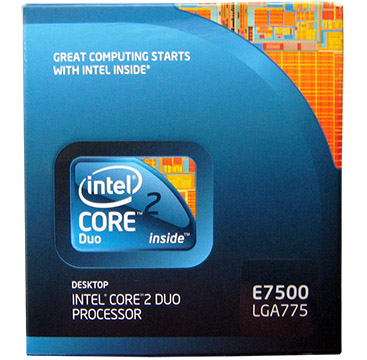
\includegraphics[width=\linewidth]{./64bit.jpg}
\end{center}
\end{column}
\begin{column}[t]{0.49\columnwidth}
New 64bit architecture!  Everyone upgrade!
\begin{itemize}
\item This was what I had in my iBook when I first came to uni
\begin{itemize}
\item (back in 2006 \texttt{:-(})
\end{itemize}
\end{itemize}

No more passing on the stack (by default)!

Loads of bits for randomisation!
\begin{block}{We're good now right\ldots{}?}
\end{block}
\end{column}
\end{columns}
\end{frame}
\begin{frame}[label={sec:orged2882d},fragile]{Randomness is still expensive though}
 \begin{lstlisting}[language=shell,numbers=none]
nm -D /usr/lib/libc.so.96.2 | wc -l
\end{lstlisting}
1679

That's a lot of symbols to randomise!
And a lot of entropy to spend at program link time\ldots{}

(Sana will cover ASLR implementation in a few weeks\ldots{})
\end{frame}
\begin{frame}[label={sec:org1ff206b},fragile]{Quick ASLR}
 So instead of loading \emph{each function} into a random location lets load \emph{each library} at a random offset!
\begin{itemize}
\item One random number per library instead of 1679.
\item You can just \texttt{mmap()} in the whole library which is \emph{fast}
\item You still don't know where the functions are \emph{precisely}
\end{itemize}

But it does mean that if a single pointer is leaked from that library, then \emph{all} the pointers are leaked
\begin{itemize}
\item You might not know where \texttt{fprintf} and \texttt{sscanf} are in memory\ldots{}
\item But you know there are precisely \texttt{b0} bytes between them
\end{itemize}
\begin{verbatim}
$ nm -nD /usr/lib/libc.so.96.2 
...
0006a900 T fprintf
0006a9b0 T sscanf
...
\end{verbatim}
\end{frame}
\begin{frame}[label={sec:orgccb9c3f},fragile]{Return to libc 2.0}
 Now to use \emph{return to libc} our attack chain is a bit more complex

\begin{enumerate}
\item Find a buffer overflow
\item Break ASLR by leaking a pointer to a library
\item Return to \texttt{main} to restart the program without re-randomising
\item Re-exploit buffer overflow to jump to the library function you now know the address of
\end{enumerate}

Its hardly arbitrary code execution though\ldots{} can we do better?
\end{frame}
\begin{frame}[label={sec:org456b4b3},fragile]{And you thought assembly was bad\ldots{}}
 \begin{columns}
\begin{column}[t]{0.79\columnwidth}
\begin{verbatim}
++++++++++[>+++++++>++++++++++>+++>+<<<<-]
>++.>+.+++++++..+++.>++.<<+++++++++++++++.
>.+++.------.--------.>+.>.
\end{verbatim}

This is \emph{brainfuck}.  It assumes memory is a big tape of \emph{cells}.
\begin{description}
\item[{\texttt{+}}] increments a cells value
\item[{\texttt{-}}] decrements a cells value
\item[{\texttt{>}}] moves to the next cell
\item[{\texttt{<}}] moves to the previous cell
\item[{\texttt{[} and \texttt{]}}] define a loop until the cell at the end is zero
\item[{\texttt{.}}] outputs the current cell value
\item[{\texttt{,}}] reads an input to the current cell
\end{description}

It is \emph{provably} Turing complete (given an infinite tape):
\begin{itemize}
\item So \emph{any} program that can be written\ldots{}
\item \emph{Could} be written in brainfuck
\end{itemize}
\end{column}
\begin{column}[t]{0.2\columnwidth}
\begin{center}
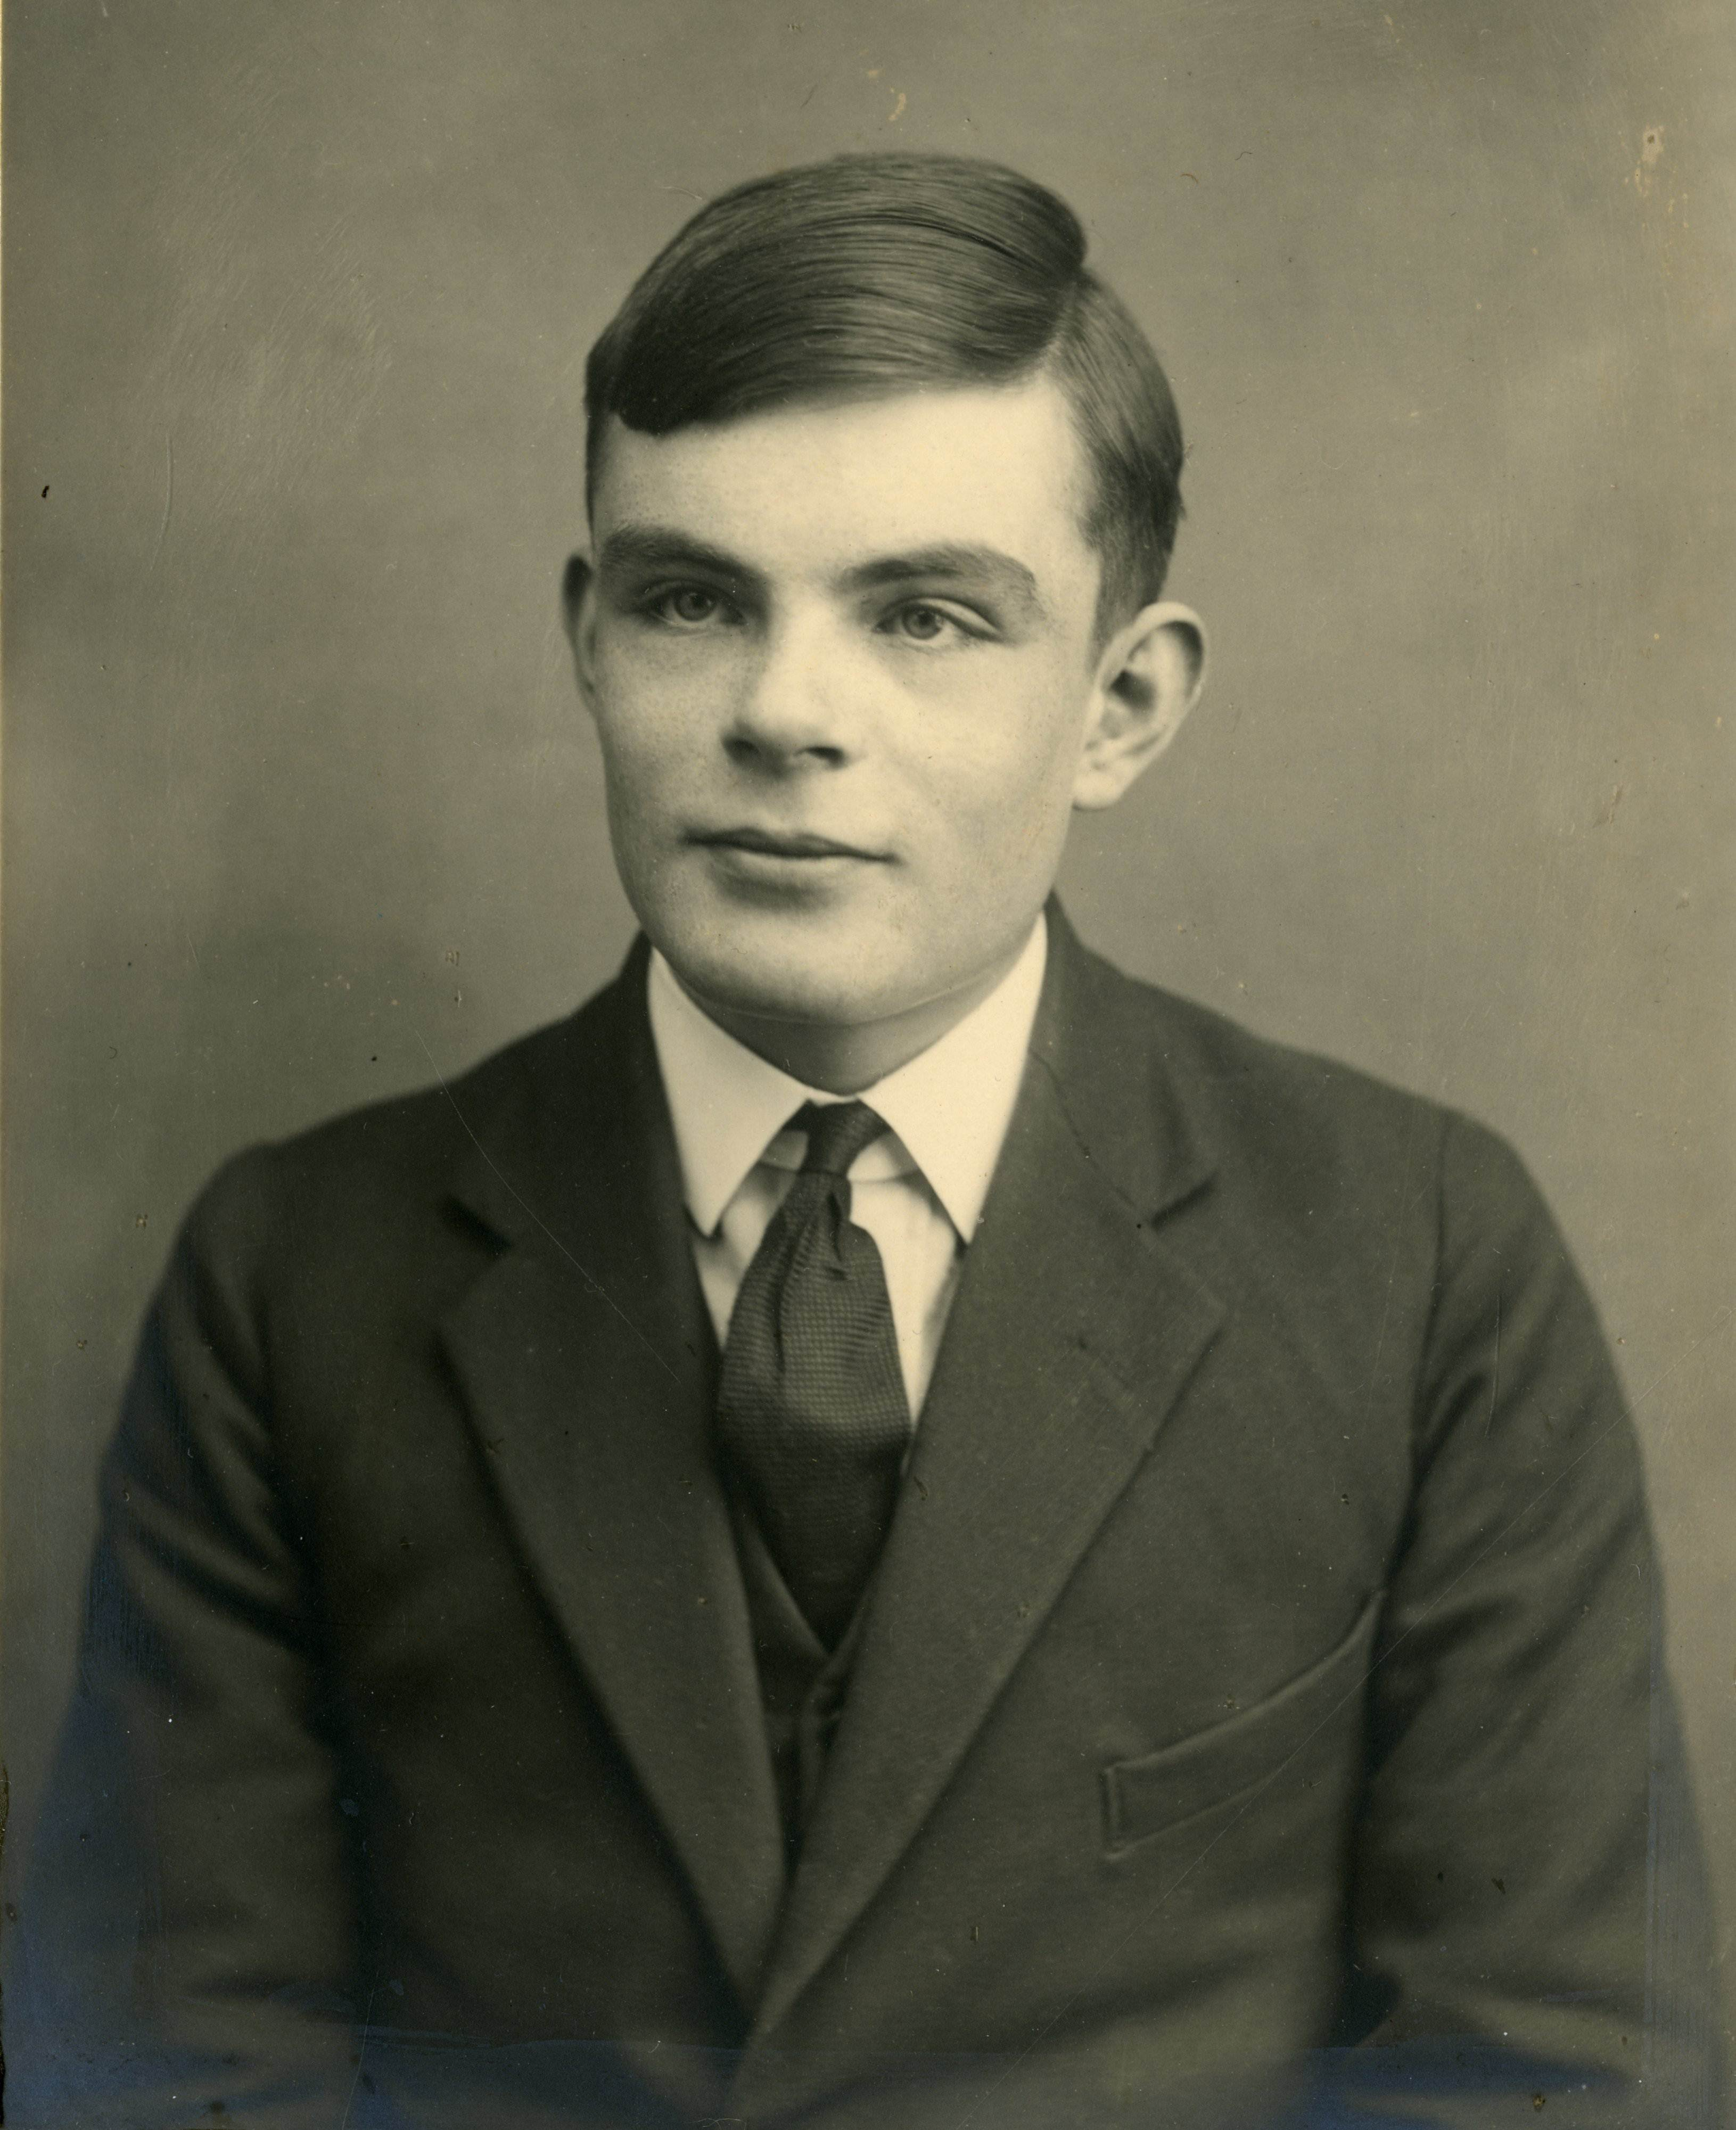
\includegraphics[width=\linewidth]{./turing.jpg}
\end{center}
\begin{center}
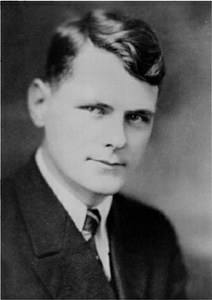
\includegraphics[width=\linewidth]{./church.jpg}
\end{center}
\end{column}
\end{columns}
\end{frame}
\begin{frame}[label={sec:org0c68c9f},fragile]{Good films start at the end}
 \begin{columns}
\begin{column}[t]{0.49\columnwidth}
Why do we need to start a function at the beginning?
\begin{itemize}
\item Functions do a bunch of interesting stuff then \texttt{ret}
\end{itemize}
\begin{block}{Return oriented programming}
A \emph{gadget} is the stuff immediately before the \texttt{ret}
\begin{itemize}
\item Typically 1 or 2 instructions
\item If we could construct a brainfuck compiler out of just these gadgets\ldots{}
\begin{itemize}
\item Then we could encode \emph{any} program as a sequence of returns through the gadgets\ldots{}
\item \ldots{}by dumping \emph{multiple} return addresses on the stack with our overflow
\end{itemize}
\end{itemize}
\end{block}
\end{column}
\begin{column}[t]{0.49\columnwidth}
\begin{lstlisting}[language=asm,numbers=none]
...
xor rax, rax
ret

...
inc rax
ret

...
inc rbx
ret

...
pop rbx
ret

...
syscall
ret
\end{lstlisting}
\end{column}
\end{columns}
\end{frame}
\begin{frame}[label={sec:orga202dc7},fragile]{Oh no\ldots{}}
 \begin{columns}
\begin{column}[t]{0.49\columnwidth}
Lets pretend we want to call \texttt{exit(0)} to crash a program early (but cleanly).
\begin{itemize}
\item \texttt{exit} is syscall number 6
\item Calling convention is syscall in \texttt{rax}, return code in \texttt{rbx}.
\end{itemize}
\begin{block}{Can we use these gadgets to make this syscall?}
\end{block}
\end{column}
\begin{column}[t]{0.49\columnwidth}
\begin{lstlisting}[language=asm,numbers=none]
  ...
xor_a:       xor rax, rax
             ret

             ...
inc_a:       inc rax
             ret

inc_b:       ...
             inc rbx
             ret

             ...
pop_b:       pop rbx
             ret

             ...
sys:         syscall
             ret
\end{lstlisting}
\end{column}
\end{columns}
\end{frame}
\begin{frame}[label={sec:org7eb32ff},fragile]{Oh no, oh no\ldots{}}
 \begin{columns}
\begin{column}[t]{0.49\columnwidth}
Lets pretend we want to call \texttt{exit(0)} to crash a program early (but cleanly).
\begin{itemize}
\item \texttt{exit} is syscall number 6
\item Calling convention is syscall in \texttt{rax}, return code in \texttt{rbx}.
\end{itemize}
\begin{block}{Can we use these gadgets to make this syscall?}
Yes! We'd just have to return back through 10 instructions!
\end{block}
\end{column}
\begin{column}[t]{0.49\columnwidth}
\begin{lstlisting}[language=asm,numbers=none]
xor_a       ; rax = 0, rbx = ?
pop_b       ; rax = 0, rbx = 0xffffffff
0xffffffff
inc_b       ; rax = 0; rbx = 0
inc_a       ; rax = 1, rbx = 0
inc_a       ; rax = 2, rbx = 0
inc_a       ; rax = 3, rbx = 0
inc_a       ; rax = 4, rbx = 0
inc_a       ; rax = 5, rbx = 0
inc_a       ; rax = 6, rbx = 0
sys         ; exit(0)
\end{lstlisting}
\end{column}
\end{columns}
\end{frame}
\begin{frame}[label={sec:org8fb26f3},fragile]{Are we really doing this? (yes)}
 Lets start with an overflow onto a return address, like we've been doing all week.

\begin{verbatim}
 <- overflown buffer 
  ----------------------
...AAA|sip |
  ----------------------
\end{verbatim}
\end{frame}
\begin{frame}[label={sec:org78a2e86},fragile]{Are we really doing this? (setup)}
 Lets stick our ROP chain on the stack

\begin{verbatim}
 <- overflown buffer 
  -------------------------------------------------------------------------
...AAA|xor_a|pop_b|FFFFFFFF|inc_b|inc_a|inc_a|inc_a|inc_a|inc_a|inc_a|sys |...
  -----^-------------------------------------------------------------------
       rsp
\end{verbatim}

And lets start returning!
\end{frame}
\begin{frame}[label={sec:org14d9b89},fragile]{Are we really doing this? (1)}
 \begin{verbatim}
rip -> xor rax, rax                rax: ?
       ret                         rbx: ?

 <- overflown buffer 
  -------------------------------------------------------------------------
...AAA|xor_a|pop_b|FFFFFFFF|inc_b|inc_a|inc_a|inc_a|inc_a|inc_a|inc_a|sys |...
  -----------^-------------------------------------------------------------
             rsp
\end{verbatim}
\end{frame}
\begin{frame}[label={sec:org1bc1082},fragile]{Are we really doing this? (2)}
 \begin{verbatim}
       xor rax, rax                rax: 0
rip -> ret                         rbx: ?

 <- overflown buffer 
  -------------------------------------------------------------------------
...AAA|xor_a|pop_b|FFFFFFFF|inc_b|inc_a|inc_a|inc_a|inc_a|inc_a|inc_a|sys |...
  -----------^-------------------------------------------------------------
             rsp
\end{verbatim}
\end{frame}
\begin{frame}[label={sec:orgcbdd5c7},fragile]{Are we really doing this? (3)}
 \begin{verbatim}
rip -> pop rbx                     rax: 0
       ret                         rbx: ?

 <- overflown buffer 
  -------------------------------------------------------------------------
...AAA|xor_a|pop_b|FFFFFFF|inc_b|inc_a|inc_a|inc_a|inc_a|inc_a|inc_a|sys |...
  -----------------^-------------------------------------------------------
                   rsp
\end{verbatim}
\end{frame}
\begin{frame}[label={sec:org00fe120},fragile]{Are we really doing this? (4)}
 \begin{verbatim}
       pop rbx                     rax: 0
rip -> ret                         rbx: FFFFFFFF

 <- overflown buffer 
  -------------------------------------------------------------------------
...AAA|xor_a|pop_b|FFFFFFF|inc_b|inc_a|inc_a|inc_a|inc_a|inc_a|inc_a|sys |...
  -------------------------^-----------------------------------------------
                           rsp
\end{verbatim}
\end{frame}
\begin{frame}[label={sec:orgcc68740},fragile]{Are we really doing this? (5)}
 \begin{verbatim}
rip -> inc rbx                     rax: 0
       ret                         rbx: FFFFFFFF

 <- overflown buffer 
  -------------------------------------------------------------------------
...AAA|xor_a|pop_b|FFFFFFF|inc_b|inc_a|inc_a|inc_a|inc_a|inc_a|inc_a|sys |...
  -------------------------------^-----------------------------------------
                                 rsp
\end{verbatim}
\end{frame}
\begin{frame}[label={sec:org4b22247},fragile]{Are we really doing this? (6)}
 \begin{verbatim}
       inc rbx                     rax: 0
rip -> ret                         rbx: 0

 <- overflown buffer 
  -------------------------------------------------------------------------
...AAA|xor_a|pop_b|FFFFFFF|inc_b|inc_a|inc_a|inc_a|inc_a|inc_a|inc_a|sys |...
  -------------------------------^-----------------------------------------
                                 rsp
\end{verbatim}
\end{frame}
\begin{frame}[label={sec:orgeea5e16},fragile]{Are we really doing this? (7)}
 \begin{verbatim}
rip -> inc rax                     rax: 0
       ret                         rbx: 0

 <- overflown buffer 
  -------------------------------------------------------------------------
...AAA|xor_a|pop_b|FFFFFFF|inc_b|inc_a|inc_a|inc_a|inc_a|inc_a|inc_a|sys |...
  -------------------------------------^-----------------------------------
                                       rsp
\end{verbatim}
\end{frame}
\begin{frame}[label={sec:org4671b21},fragile]{Are we really doing this? (8)}
 \begin{verbatim}
       inc rax                     rax: 1
rip -> ret                         rbx: 0

 <- overflown buffer 
  -------------------------------------------------------------------------
...AAA|xor_a|pop_b|FFFFFFF|inc_b|inc_a|inc_a|inc_a|inc_a|inc_a|inc_a|sys |...
  -------------------------------------^-----------------------------------
                                       rsp
\end{verbatim}
\end{frame}
\begin{frame}[label={sec:orgdd7c553},fragile]{Are we really doing this? (9)}
 \begin{verbatim}
rip -> inc rax                     rax: 1
       ret                         rbx: 0

 <- overflown buffer 
  -------------------------------------------------------------------------
...AAA|xor_a|pop_b|FFFFFFF|inc_b|inc_a|inc_a|inc_a|inc_a|inc_a|inc_a|sys |...
  -------------------------------------------^-----------------------------
                                             rsp
\end{verbatim}
\end{frame}
\begin{frame}[label={sec:org4c306dd},fragile]{Are we really doing this? (10)}
 \begin{verbatim}
       inc rax                     rax: 2
rip -> ret                         rbx: 0

 <- overflown buffer 
  -------------------------------------------------------------------------
...AAA|xor_a|pop_b|FFFFFFF|inc_b|inc_a|inc_a|inc_a|inc_a|inc_a|inc_a|sys |...
  -------------------------------------------^-----------------------------
                                             rsp
\end{verbatim}
\end{frame}
\begin{frame}[label={sec:org8b55925},fragile]{Are we really doing this? (11)}
 \begin{verbatim}
rip -> inc rax                     rax: 2
       ret                         rbx: 0

 <- overflown buffer 
  -------------------------------------------------------------------------
...AAA|xor_a|pop_b|FFFFFFF|inc_b|inc_a|inc_a|inc_a|inc_a|inc_a|inc_a|sys |...
  -------------------------------------------------^-----------------------
                                                   rsp
\end{verbatim}
\end{frame}
\begin{frame}[label={sec:orgf6ec11d},fragile]{Are we really doing this? (12)}
 \begin{verbatim}
       inc rax                     rax: 3
rip -> ret                         rbx: 0

 <- overflown buffer 
  -------------------------------------------------------------------------
...AAA|xor_a|pop_b|FFFFFFF|inc_b|inc_a|inc_a|inc_a|inc_a|inc_a|inc_a|sys |...
  -------------------------------------------------^-----------------------
                                                   rsp
\end{verbatim}
\end{frame}
\begin{frame}[label={sec:org28d2cd0},fragile]{Are we really doing this? (13)}
 \begin{verbatim}
rip -> inc rax                     rax: 3
       ret                         rbx: 0

 <- overflown buffer 
  -------------------------------------------------------------------------
...AAA|xor_a|pop_b|FFFFFFF|inc_b|inc_a|inc_a|inc_a|inc_a|inc_a|inc_a|sys |...
  -------------------------------------------------------^-----------------
                                                         rsp
\end{verbatim}
\end{frame}
\begin{frame}[label={sec:org9850fcc},fragile]{Are we really doing this? (14)}
 \begin{verbatim}
       inc rax                     rax: 4
rip -> ret                         rbx: 0

 <- overflown buffer 
  -------------------------------------------------------------------------
...AAA|xor_a|pop_b|FFFFFFF|inc_b|inc_a|inc_a|inc_a|inc_a|inc_a|inc_a|sys |...
  -------------------------------------------------------^-----------------
                                                         rsp
\end{verbatim}
\end{frame}
\begin{frame}[label={sec:org8e35ac5},fragile]{Are we really doing this? (15)}
 \begin{verbatim}
rip -> inc rax                     rax: 4
       ret                         rbx: 0

 <- overflown buffer 
  -------------------------------------------------------------------------
...AAA|xor_a|pop_b|FFFFFFF|inc_b|inc_a|inc_a|inc_a|inc_a|inc_a|inc_a|sys |...
  -------------------------------------------------------------^-----------
                                                               rsp
\end{verbatim}
\end{frame}
\begin{frame}[label={sec:orgdc63154},fragile]{Are we really doing this? (16)}
 \begin{verbatim}
       inc rax                     rax: 5
rip -> ret                         rbx: 0

 <- overflown buffer 
  -------------------------------------------------------------------------
...AAA|xor_a|pop_b|FFFFFFF|inc_b|inc_a|inc_a|inc_a|inc_a|inc_a|inc_a|sys |...
  -------------------------------------------------------------^-----------
                                                               rsp
\end{verbatim}
\end{frame}
\begin{frame}[label={sec:org470a36e},fragile]{Are we really doing this? (17)}
 \begin{verbatim}
rip -> inc rax                     rax: 5
       ret                         rbx: 0

 <- overflown buffer 
  -------------------------------------------------------------------------
...AAA|xor_a|pop_b|FFFFFFF|inc_b|inc_a|inc_a|inc_a|inc_a|inc_a|inc_a|sys |...
  -------------------------------------------------------------------^-----
                                                                     rsp
\end{verbatim}
\end{frame}
\begin{frame}[label={sec:org02f7f1c},fragile]{Are we really doing this? (18)}
 \begin{verbatim}
       inc rax                     rax: 6
rip -> ret                         rbx: 0

 <- overflown buffer 
  -------------------------------------------------------------------------
...AAA|xor_a|pop_b|FFFFFFF|inc_b|inc_a|inc_a|inc_a|inc_a|inc_a|inc_a|sys |...
  -------------------------------------------------------------------^-----
                                                                     rsp
\end{verbatim}
\end{frame}
\begin{frame}[label={sec:org7177781},fragile]{Are we really doing this? (19)}
 \begin{verbatim}
rip -> syscall                     rax: 6
                                   rbx: 0

 <- overflown buffer 
  -------------------------------------------------------------------------
...AAA|xor_a|pop_b|FFFFFFF|inc_b|inc_a|inc_a|inc_a|inc_a|inc_a|inc_a|sys |...
  ------------------------------------------------------------------------^
                                                                          rsp
\end{verbatim}

Woohoo! \texttt{exit(0)} is called!
\end{frame}
\begin{frame}[label={sec:org3b58f29},fragile]{Return Oriented Programming}
 We just wrote an entire program by writing our shellcode as a path through pre-existing code in our program
\begin{itemize}
\item Arbitrary code execution purely through reuse!
\item Most sufficiently large programs will contain enough usable gadgets that arbitrary code can be loaded
\end{itemize}

This is \emph{(pretty much)} the state of the art for arbitrary code execution via a buffer overflow
\begin{itemize}
\item (\emph{ish\ldots{}} there's JOP too which is similar but for case statements)
\end{itemize}

We're going to be trying this \emph{in practice} for next week's lab \texttt{:-D}
\end{frame}
\begin{frame}[label={sec:org0af9d2e}]{How do we stop this?}
\end{frame}
\begin{frame}[label={sec:orgf25b715}]{How do we stop this?}
We can't trivially.

ROP falls out from fundamental decisions about how computers were architected that we made back in the 60s
\begin{itemize}
\item Von Neumann vs Harvard architectures
\end{itemize}

There are techniques that we can use to make it harder though
\begin{description}
\item[{Shadow stacks}] keep a second stack for stack consistency checking and have the kernel kill the program if it ever gets out of sync
\item[{Full ASLR}] really randomise everything
\item[{Instruction Pointer Integrity Protections}] on return check that our instruction pointer goes only to whitelisted addresses (or is aligned)
\end{description}
\end{frame}
\begin{frame}[label={sec:org49a9d42}]{How do we stop this?}
\ldots{}maybe we should just fix the buffer overflow?
\begin{itemize}
\item Rust/Zig!
\item Not using unsafe languages

\vfill
\end{itemize}
\emph{(But wheres the fun in that?)}
\end{frame}
\begin{frame}[label={sec:org7221437}]{Recap}
We went from:
\begin{itemize}
\item buffer overflows in the 90s\ldots{}
\item \ldots{}up to ROP in the 20s
\end{itemize}

All that CS theory you learned in first year is actually useful for something.

There are worse ways of programming than assembly language!
\begin{block}{Next time}
\begin{description}
\item[{In the lab}] ROP
\item[{Lectures}] Sana's taking over for a few weeks!
\end{description}

(I'll be back once more to talk about why computer hardware is fundamentally broken and why we should all be very depressed)
\end{block}
\end{frame}
\end{document}